\hspace{0.5cm} This paper employs a dataset of Spanish business news articles sourced from Dow Jones Newswires, covering the period from June 24, 2020, to September 30, 2021. The selection of this timeframe is deliberate, driven by two key considerations. 
%
First, given the substantial computational demands of LLM-based analysis, we strategically focus on a smaller, carefully curated dataset. This deliberate scope reduction allows us to thoroughly demonstrate our novel methodology's effectiveness in decoding market-news relationships while keeping computational costs manageable. Rather than pursuing a broad-scale analysis, we prioritize proving our approach's utility through a focused, computationally feasible study that can serve as a foundation for future expansions.
%
%First, we aim to test a novel methodology on a relatively small dataset to ensure feasibility and demonstrate its utility in understanding market reactions to news. Our goal is not to conduct a big data analysis, but rather to showcase the methodology's potential on a manageable dataset. 
%
Second, we specifically chose the Covid-19 era to test our methodology's extrapolative capabilities during periods of significant market instability and volatility. While existing textual algorithms typically perform well in stable market conditions, they often struggle to generalize effectively during periods of heightened uncertainty. By focusing on this volatile period, we can better assess our methodology's robustness and its ability to maintain predictive power under challenging market conditions.
%Second, to evaluate the extrapolative power of the proposed methodology, it is important that the data span a period characterized by instability and volatility, which is why we focus on the Covid-19 era. Notably, textual algorithms are able to extrapolate well out of sample under relatively stable time periods, however, when challenged in uncertain or volatile periods, they tend to fail to generalize well out of sample.

The dataset consists of high-quality articles that have been filtered to include only those mentioning Spanish publicly traded firms listed on the IBEX-35 index. These 35 companies represent the largest firms in Spain by market capitalization and are typically the most liquid and actively traded Spanish stocks. Moreover, these companies tend to receive the most consistent media coverage, making them ideal for the scope of our analysis.

The use of Dow Jones Newswires as our news source is also intentional. Dow Jones has a standard practice of including the stock market ticker of firms directly affected by the article in parentheses, while excluding firms mentioned for secondary purposes from ticker specification.
This feature significantly facilitates the extraction of named entities (i.e., Named Entity Recognition, or NER). The tickers used by Dow Jones align with those from Yahoo Finance, enabling seamless integration between our NER algorithm and subsequent firm-specific trading operations via the Yahoo Finance API.
%
We employ a pattern recognition algorithm through the \texttt{regex} library in Python to identify specific mentions of publicly traded companies in the Spanish stock exchange. The algorithm searches for patterns of the form ``\texttt{(<WORD>.MC)}'' for any \texttt{<WORD>}. For instance, consider the following example article (translated into English for convenience):
%Specifically, we employ a pattern recognition algorithm (through the \texttt{regex} library in Python) to identify specific mentions to publicly traded companies in the Spanish stock exchange by searching for patterns of the form ``\texttt{(<WORD>.MC)}'' for any \texttt{<WORD>}. For instance, consider the following example article (translated into English for convenience):


\begin{news}
[An article about ACS and Acciona]
[news:article-acs-acciona]
{ACS and Acciona Secure Contracts for New Australian Airport 
%Worth EUR164 Million
}
A consortium of Actividades de Construcci�n y Servicios SA \red{(ACS.MC)} and Acciona SA \red{(ANA.MC)} has won a contract to build the operations area of the Western Sydney International Airport (Nancy-Bird Walton) and carry out paving works, amounting to AUD265 million (EUR164 million) for the Australian subsidiary CIMIC Group Ltd (CIM.AU). CIMIC will carry out the work through its subsidiary CPB Contractors, as stated in a press release. This is the third project awarded by Western Sydney Airport to the joint venture after being selected to carry out earthworks.
%The scope of the works includes paving of runways and taxiways, aircraft isolation platforms, lateral roads, landscaping, aeronautical lighting systems, associated buildings of the electrical substation, as well as other specialized systems.
Construction will take two years, and the Western Sydney airport is expected to open in 2026.	
\end{news}


%\begin{news}
%[A news article about d]
%[news:dfdf]
%{CaixaBank Leads EUR1,000 Million Sustainable Loan for Naturgy}
%CaixaBank SA (CABK.MC) reported on Wednesday that it is leading a syndicated loan for the energy group Naturgy Energy Group SA (NTGY.MC) amounting to EUR1,000 million with a three-year maturity. This sustainable financing includes objectives for reducing greenhouse gas emissions. The bank stated in a press release that it has acted as coordinator in this loan, which also involves Banco Bilbao Vizcaya Argentaria SA (BBVA.MC) and Banco Santander SA (SAN.MC). This financing complements the green loan formalized by Naturgy in 2019 and the issuance of a green bond in 2017, operations also led by CaixaBank, the entity indicated.
%\end{news}

%\begin{news}
%[]
%[]
%{
%Spain's Inclusion in German Risk Zones List Will Have Limited Impact
%}
%The decision by Germany to add all of Spain to its list of risk zones will have a \qquote{limited impact, as, for now, only travel advisories have been issued and the requirements, if traveling to Spain, are reduced to taking a negative PCR test upon return or a complete immunization test,} Sabadell states. However, \qquote{if this changes and new restrictions are announced, it would be very negative for hotel companies}, especially for Meli� (MEL.MC), particularly if it affects the Balearic and Canary Islands, the entity indicates. \qquote{It would leave recovery in the hands of national demand, which represents only around 30\% of total overnight stays,} it points out. German tourism accounts for 11\% of Meli�'s EBIT. In contrast, for NH (NHH.MC) the possible effect \qquote{is residual} due to its urban hotel business model, says Sabadell, which also does not foresee a potential impact for IAG (IAG.MC).
%\end{news}


%\begin{news}
%    [A news article about Telef�nica and Cellnex]  
%    [news:cellnex-article]                            
%    {Cellnex will face more competition in Europe} Telef�nica's \red{(TEF.MC)} subsidiary, Telxius Telecom, has agreed to sell its telecommunications tower division in Europe and Latin America to American Tower (AMT), which will expand the latter's presence in Europe and increase competition for the Spanish wireless telecommunications group Cellnex Telecom \red{(CLNX.MC)}, according to Equita Sim. The transaction "represents the entry of a new independent tower operator into the Spanish market and potentially more competition for future growth in the European market as well," says the brokerage firm.
%\end{news}

Our NER algorithm applied to  Article \ref{news:article-acs-acciona} successfully identifies the Spanish firms \texttt{ACS.MC} (Actividades de Construcci�n y Servicios SA) and \texttt{ANA.MC} (Acciona SA) while disregarding the Australian \texttt{CIM.AU} (CIMIC Groups Ltd). 
To further ensure the reliability of firm identification, we validate the extracted entities using a Large Language Model (LLM).
%To enhance the reliability of firm identification, we further validate the extracted entities using a Large Language Model (LLM).
In particular, we feed the articles to the LLM, which parses them according to a predefined schema. As we will see later, the first task in this schema 
is to identify the listed Spanish firms directly affected by the events described in the article. Finally, the identified firms are filtered against a dynamic list of IBEX-35 members.
%is to identify all the Spanish firms listed on the IBEX-35 that are directly affected by the shocks described in the news article. 
Due to the high quality of the dataset, the correlation between entities identified by the LLM and those extracted via pattern recognition is almost exact.

For subsequent analysis, we partition the dataset into three splits: \textit{Train}, \textit{Validation}, and \textit{Test}. Each split serves a distinct purpose that will be explained in detail as we progress through the paper. Summary statistics for each data split are provided in \cref{tab:Articles_Summary_Statistics}.

%----------------------------------------------------
\inserthere{tab:Articles_Summary_Statistics}

\begin{table}[H]
\centering
\caption{Summary Statistics of Articles by Data Split}
\label{tab:Articles_Summary_Statistics}
%\begin{tabular}{|l||c|c|c|c|}
\begin{tabular}{lcccc}
\hline \Xhline{2\arrayrulewidth}
%\rowcolor{gray!10}
\textbf{Data Split} & \textbf{Time Period} & \textbf{\# Articles} & \textbf{\# Words} & \textbf{Vocabulary Size} \\
\hline \Xhline{2\arrayrulewidth}
Train & 24/06/2020 $-$ 12/02/2021 & 1254 & 327413 & 26762 \\
Validation & 12/02/2021 $-$ 21/06/2021 & 836 & 232912 & 22265 \\
Test & 21/06/2021 $-$ 30/09/2021 & 523 & 140495 & 16474 \\ \hline \Xhline{\arrayrulewidth}
All & 24/06/2020 $-$ 30/09/2021 & 2613 & 700820 & 42603 \\ \hline \Xhline{2\arrayrulewidth}
\end{tabular}
\mx 
\subcaption*{\textit{Note: Summary statistics by data splits and for the whole sample. We provide the period spanned by each data split, the number of articles, the number of words, and the vocabulary size. Articles have been preprocessed following standard NLP practices.}}
\end{table}

%----------------------------------------------------

The most frequently used words in the whole dataset are depicted in \cref{fig:WordCloud} by means of a WordCloud. As shown, the most prominent words include \qquote{empresa} (firm), \qquote{compa��a} (company), and \qquote{espa�a} (Spain), reinforcing that the dataset primarily comprises Spanish business news, with a prevalence of technical terms such as \qquote{beneficio neto} (net profit), \qquote{precio objetivo} (target price), \qquote{proyecto} (project), and \qquote{operaci�n} (operation).

%----------------------------------------------------
\inserthere{fig:WordCloud}
\begin{figure}[H]
  \centering
  \caption{Word Cloud of all the dataset}
  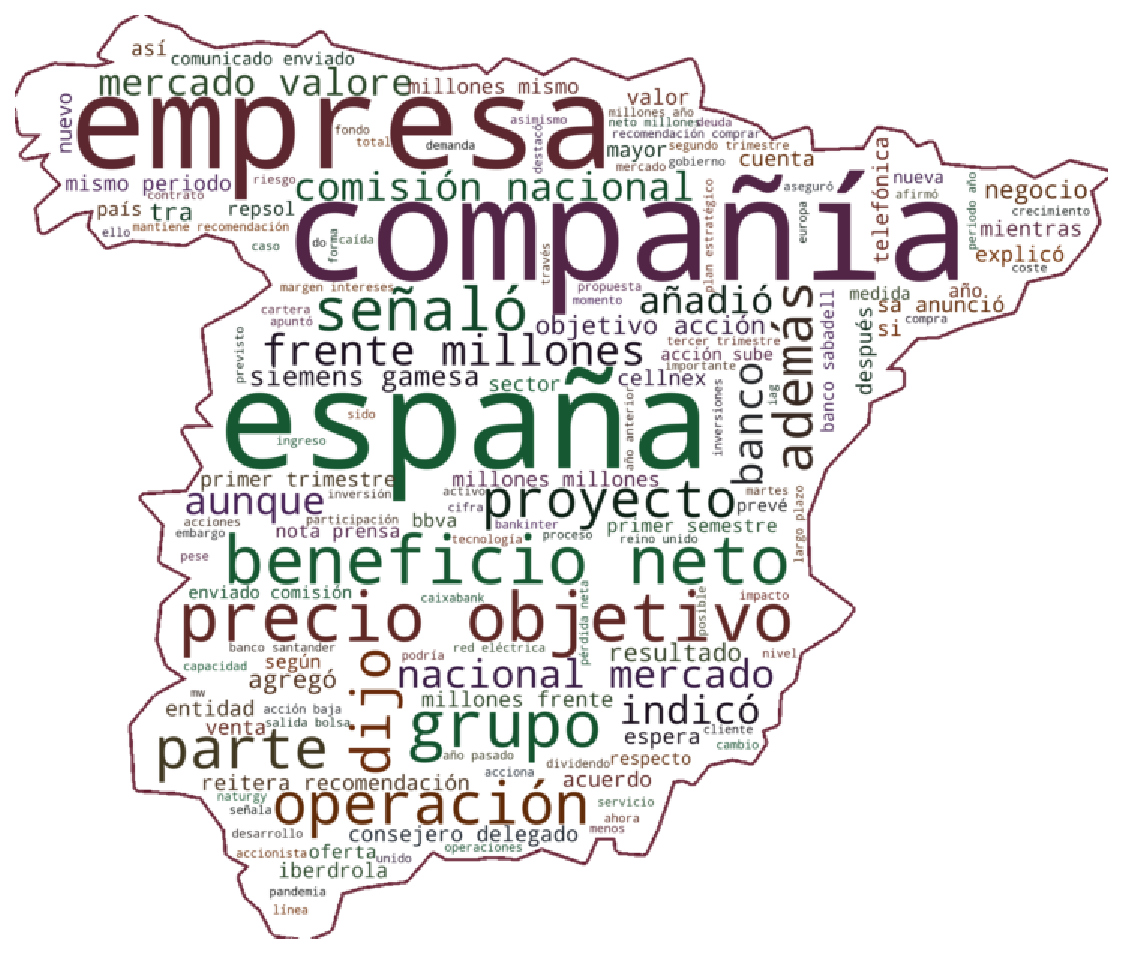
\includegraphics[scale=0.496]{/Users/jesusvillotamiranda/Library/CloudStorage/OneDrive-UniversidaddeLaRioja/CEMFI/__MSc__/__Second_year__/6th_Term/MasterThesis/__Output/EDA_WordCloud.pdf}
  \label{fig:WordCloud}
  \subcaption*{\textit{Note: This Word Cloud visualizes the most frequent words in our dataset of Spanish business news articles. Larger words correspond to higher frequencies. The color of the words is purely for visual differentiation and holds no additional meaning. The most prominent words include \qquote{empresa} (firm), \qquote{compa��a} (company), and \qquote{espa�a} (Spain), reinforcing that the dataset primarily comprises Spanish business news, with a prevalence of technical terms such as \qquote{beneficio neto} (net profit), \qquote{precio objetivo} (target price), \qquote{proyecto} (project), and \qquote{operaci�n} (operation).}}
\end{figure}
%----------------------------------------------------

The distribution of the number of articles published per day is illustrated in \cref{fig:hist_1}, showing that the most frequent publication rate is between 5 and 10 articles per day, though some days exhibit unusually high publication counts. \cref{fig:hist_2} shows the distribution of the number of words per article, with the majority of articles containing between 70 and 280 words. This indicates that the articles are relatively succinct, providing direct information. 
However, the long right tail points to instances of more comprehensive coverage.
%However, a small subset of articles exceeds 500 words, indicating more in-depth coverage.

%----------------------------------------------------
\inserthere{fig:histograms}
\begin{figure}[H]
  \caption{Histogram of \# News Articles per Day and \# Words per Article}
  \centering
  \begin{subfigure}[b]{0.46\textwidth}
    \centering
    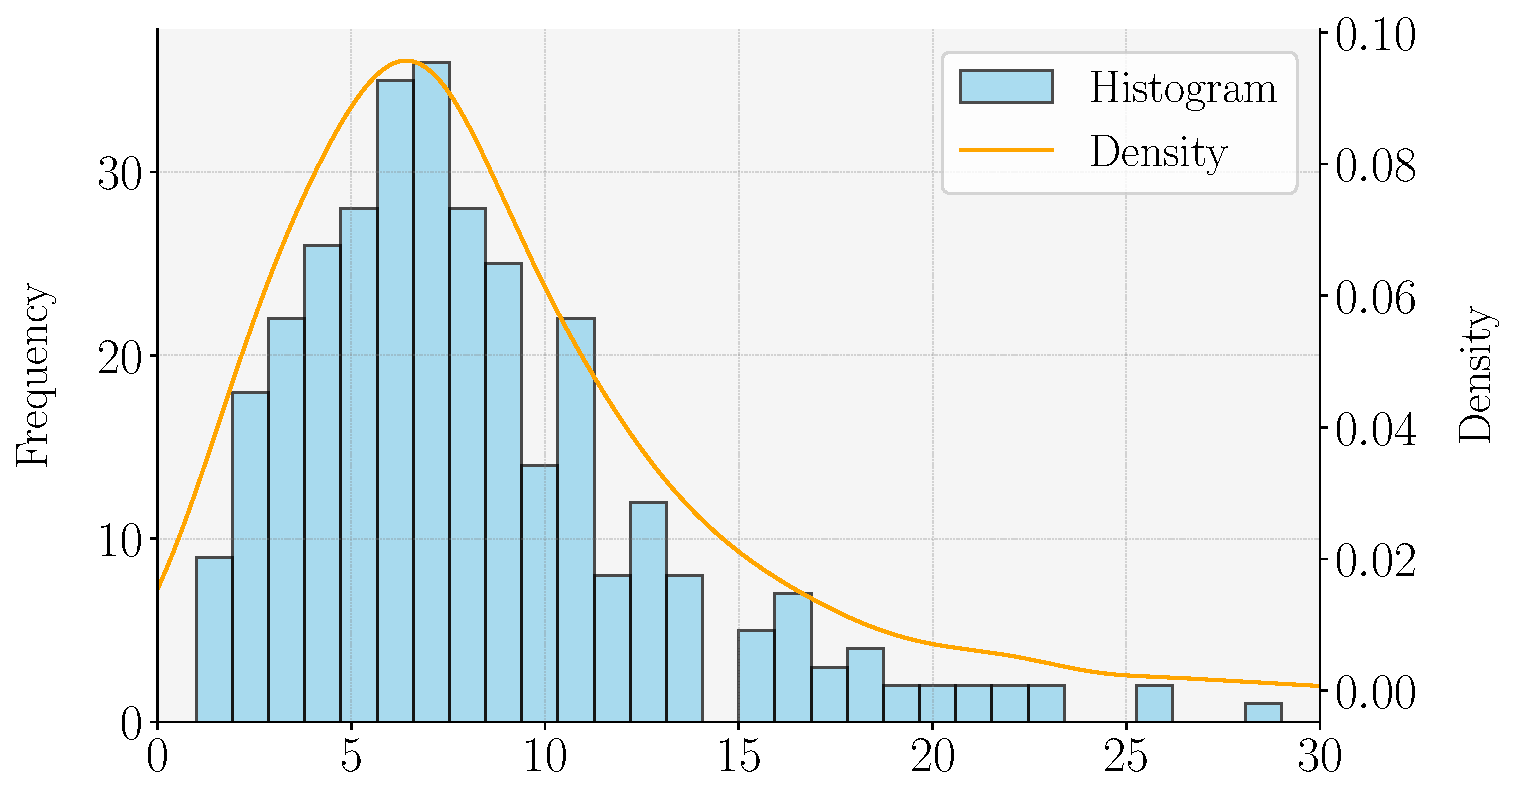
\includegraphics[width=\textwidth]{/Users/jesusvillotamiranda/Library/CloudStorage/OneDrive-UniversidaddeLaRioja/CEMFI/__MSc__/__Second_year__/6th_Term/MasterThesis/__Output/EDA_Histogram_of_Number_of_News_Articles_per_day.pdf}
    \caption{Number of News Articles per Day}
    \label{fig:hist_1}
  \end{subfigure}
  \hspace{0.05\textwidth} % Add horizontal space between the subfigures
  \begin{subfigure}[b]{0.46\textwidth}
    \centering
    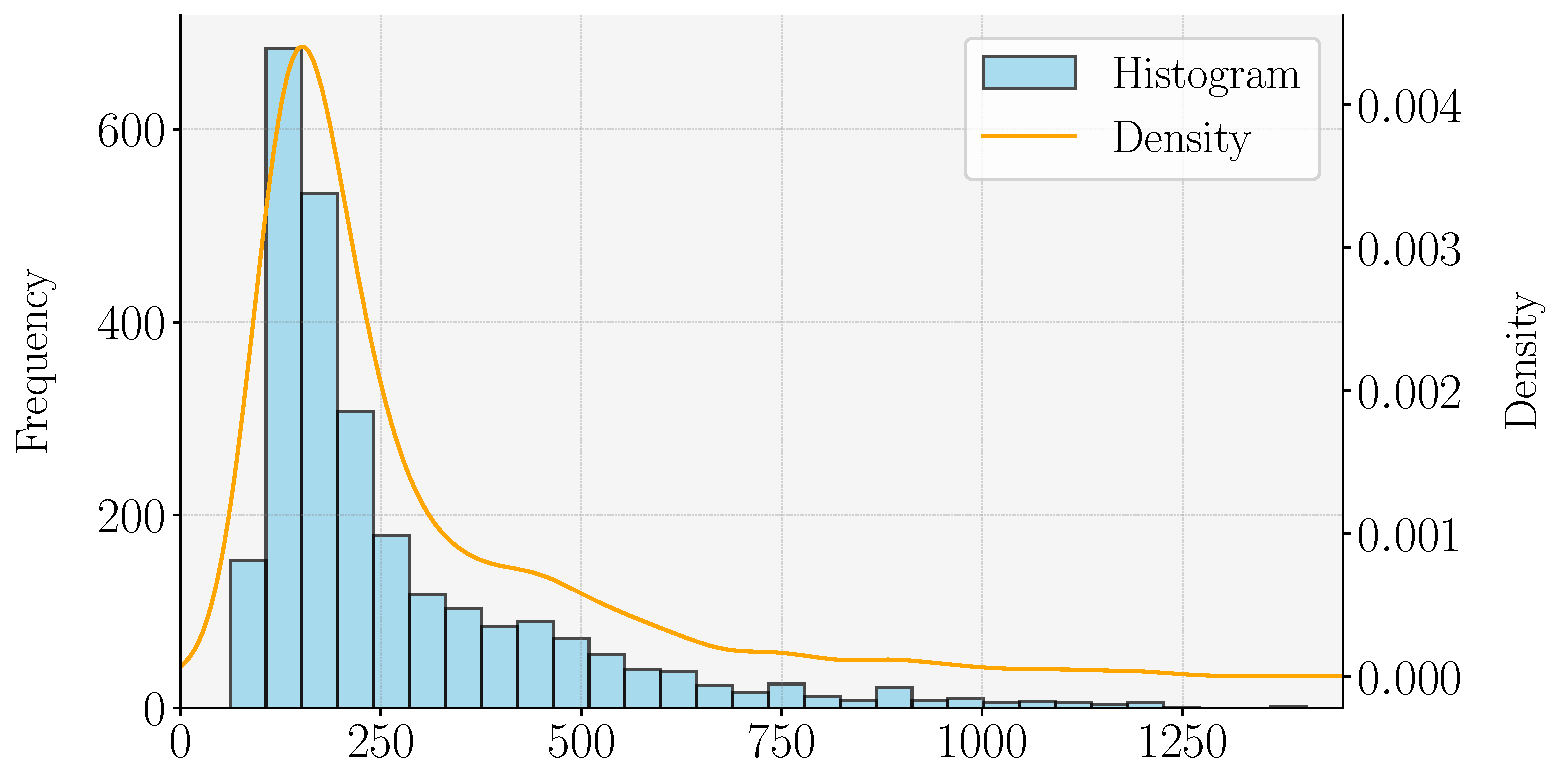
\includegraphics[width=\textwidth]{/Users/jesusvillotamiranda/Library/CloudStorage/OneDrive-UniversidaddeLaRioja/CEMFI/__MSc__/__Second_year__/6th_Term/MasterThesis/__Output/EDA_Number_of_Words_per_Article.pdf}
    \caption{Number of Words per Article}
    \label{fig:hist_2}
  \end{subfigure}
  \label{fig:histograms}
  \subcaption*{\textit{Note: Panel (a) displays the distribution of the number of news articles published per day, with most days having between 5 and 10 articles. Panel (b) shows the distribution of the number of words per article, where the majority are between 70 and 280 words, suggesting concise reporting. However, the long right tail indicates instances of more comprehensive coverage.}}

\end{figure}
%----------------------------------------------------

The time series of the number of articles published per day throughout the sample period is shown in \Cref{fig:ts_articles}. The series exhibits considerable variability, with frequent fluctuations from fewer than 5 articles per day to sudden spikes exceeding 20 articles. The 30-day moving average smooths the series, confirming the previous observation that, on average, between 5 and 10 articles are published daily.

%----------------------------------------------------
\inserthere{fig:ts_articles}
\begin{figure}[H]
  \centering
  \caption{Time Series of Number of Articles per Day and 30-Period Moving Average}
  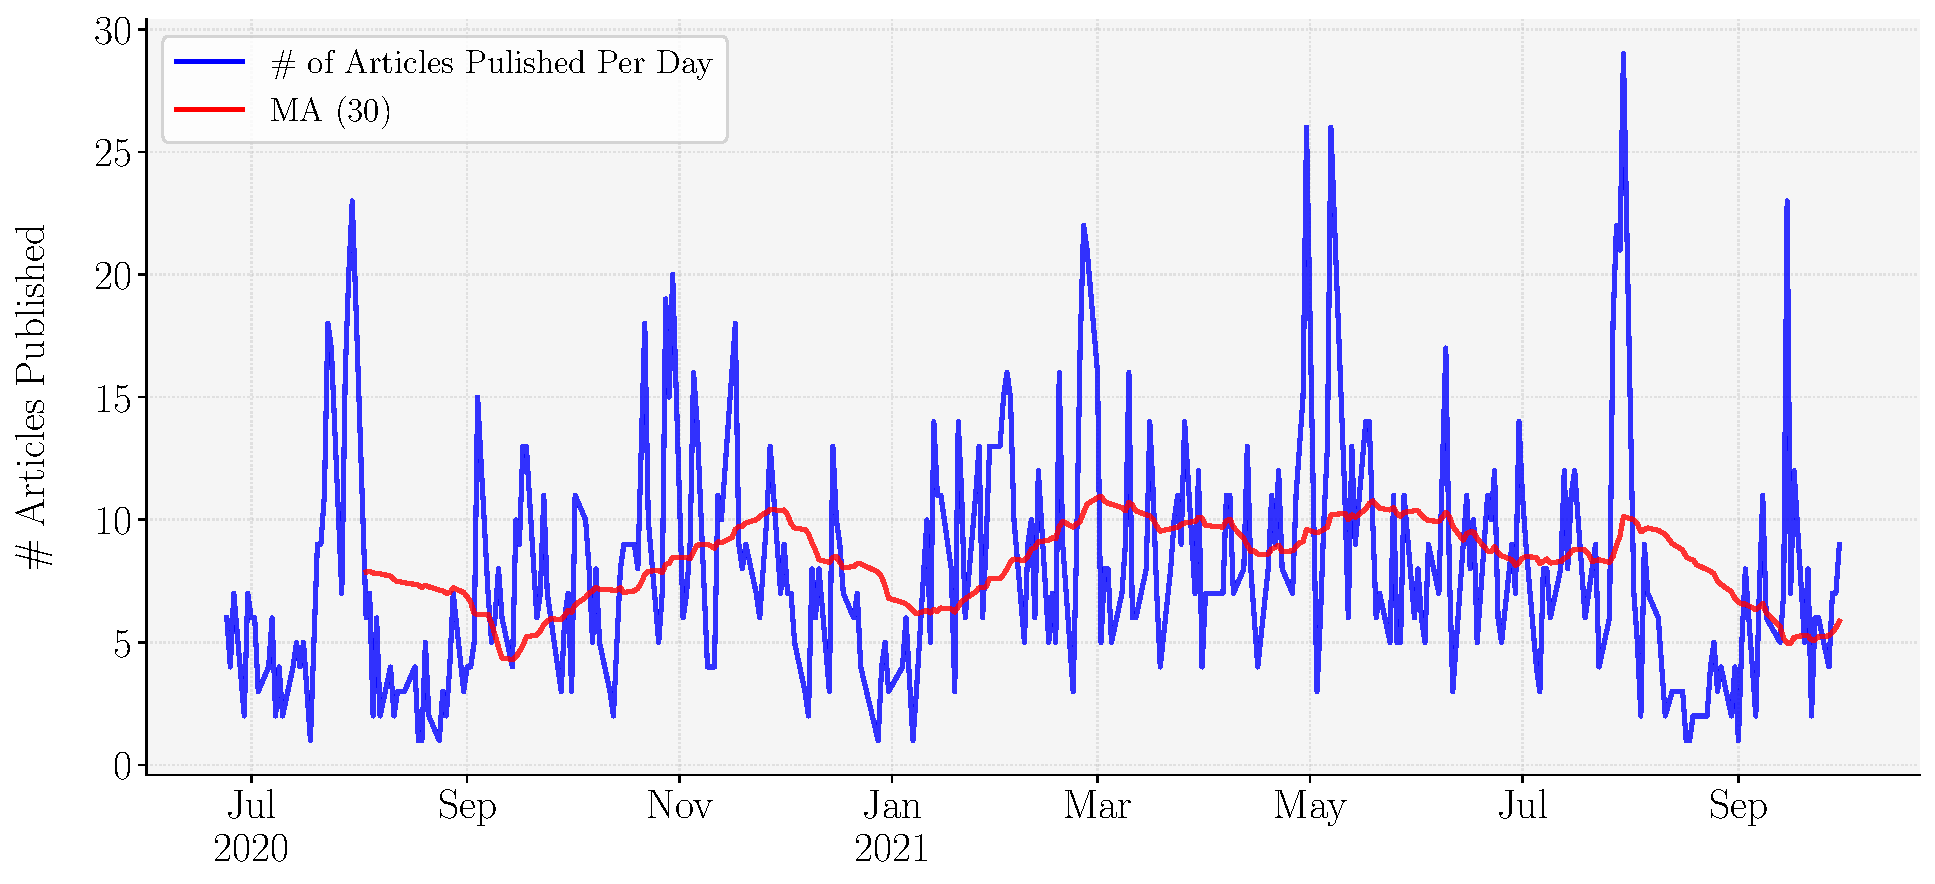
\includegraphics[scale=0.445]{/Users/jesusvillotamiranda/Library/CloudStorage/OneDrive-UniversidaddeLaRioja/CEMFI/__MSc__/__Second_year__/6th_Term/MasterThesis/__Output/EDA_Time_Series_of_Articles.pdf}
  \label{fig:ts_articles}
  \subcaption*{\textit{Note: The time series shows the daily number of news articles published, characterized by significant variability with occasional sharp spikes. The 30-day moving average smooths these fluctuations, revealing an average publication rate of 5 to 10 articles per day.}}
\end{figure}
%----------------------------------------------------